\documentclass[12pt]{article}

\usepackage{bm}
\usepackage{amsmath}
\usepackage{amssymb}
\usepackage{undertilde}
\usepackage{esint}
\usepackage{graphicx}
\usepackage{float}
\usepackage{enumitem}
\usepackage{mathtools}


\usepackage{listings}
\usepackage{color}

\definecolor{dkgreen}{rgb}{0,0.6,0}
\definecolor{gray}{rgb}{0.5,0.5,0.5}
\definecolor{mauve}{rgb}{0.58,0,0.82}
\setlength{\textheight}{24cm}
\setlength{\parskip}{0.5cm}    % Gap between paragraphs
\setlength{\parindent}{0cm}     % Suppresses indents on new paragraphs
\setlength{\topmargin}{-1.5cm}

\DeclarePairedDelimiter\floor{\lfloor}{\rfloor}
\DeclareMathOperator{\sgn}{sgn}

\lstset{frame=tb,
  language=Java,
  aboveskip=1mm,
  belowskip=1mm,
  showstringspaces=false,
  columns=flexible,
  basicstyle={\tiny\ttfamily},
  numbers=none,
  commentstyle=\color{dkgreen},
  stringstyle=\color{red},
  emph={int,char,double,float,long, void,boolean, Integer, import, public, class, for, static, main, String, Random, new, if},
  emphstyle={\color{blue}},
  escapechar=\&,
  classoffset=1, % starting new class
  otherkeywords={>,<,.,;,-,!,=,~},
    morekeywords={>,<,.,;,-,!,=,~},
    keywordstyle=\color{red},
    classoffset=0,
  numberstyle=\tiny\color{gray},
  stringstyle=\color{mauve},
  breaklines=true,
  breakatwhitespace=true,
  tabsize=4
}

\parindent = 3mm
\unitlength=3mm

\setlength{\textwidth}{183.0truemm}
\setlength{\textheight}{245.0truemm}
\setlength{\oddsidemargin}{-8.0mm}
\setlength{\evensidemargin}{-8.0mm}
\setlength{\topmargin}{-20.5truemm}
\setlength{\belowcaptionskip}{-10pt}

\begin{document}

\begin{center}
\textbf{COMP3506 \\ Assignment 2 Question 2 \\ Name: Adrian Rahul Kamal Rajkamal \\ Student Number: 45811935 \\ Tutorial Group: T10 (Wednesday 12pm)}
\end{center}

\vskip 0.2cm

Tables \ref{table:unsorted}-\ref{table:descending} present the runtimes (in milliseconds) found for each of the test cases, in each of the three situations.

Figures \ref{fig:unsorted}-\ref{fig:reverse} present plots of these runtimes against array length.

\begin{center}
\begin{table}[H]
$$\begin{array}{|c|c|c|c|c|c|c|c|}\hline
\textbf{Algorithm} & n=5 & n=10 & n=50 & n=100 & n=500 & n=1000 & n=10000 \\ \hline
\text{Selection Sort}& 0.0026 & 0.0075 & 0.0915 & 0.4643 & 7.0129 & 18.8858 & 238.0944 \\ \hline
\text{Insertion Sort}& 0.0042 & 0.0052 & 0.0622 & 0.4971 & 4.4076 & 10.4359 & 225.6123\\ \hline
\text{Merge Sort} & 0.0104 & 0.0297 & 0.0896 & 0.174 & 1.1387 & 2.1514 & 6.2014 \\ \hline
\text{Quick Sort}& 0.0097 & 0.0293 & 0.0845 & 0.1864 & 1.6774 & 2.6933 & 23.5392 \\ \hline
\end{array}$$
\caption{Runtime Performance of Random Unsorted Numbers}
\label{table:unsorted}
\end{table}

\begin{center}
\begin{figure}[H]
\hfill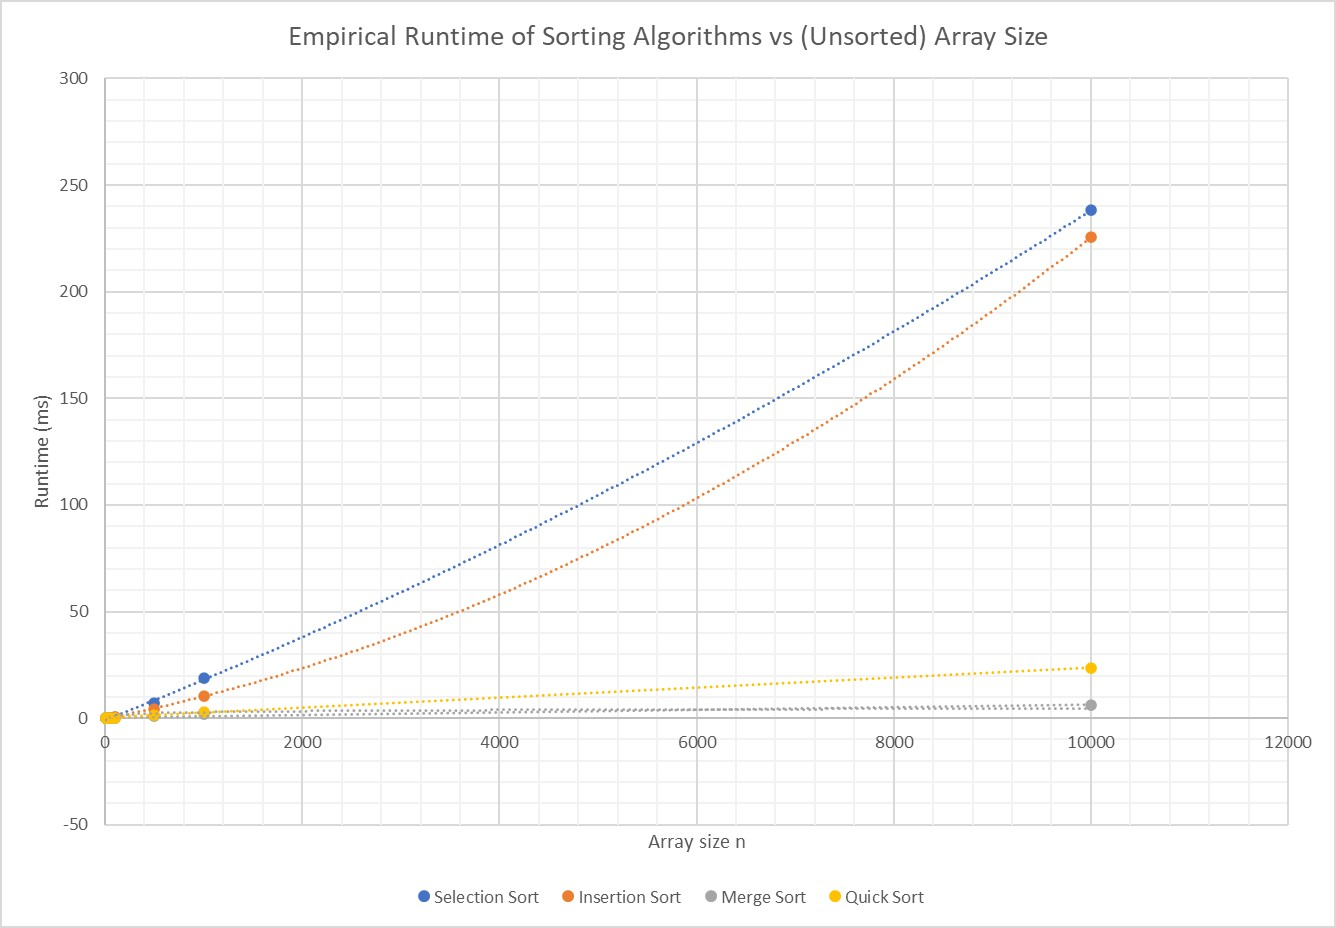
\includegraphics[scale=0.8]{unsorted.jpg}
\hspace*{\fill}
\caption{Runtime vs Array Size for Different Sorting Algorithms on Unsorted Arrays}
\label{fig:unsorted}
\end{figure}
\end{center}

\begin{table}[H]
$$\begin{array}{|c|c|c|c|c|c|c|c|}\hline
\textbf{Algorithm} & n=5 & n=10 & n=50 & n=100 & n=500 & n=1000 & n=10000 \\ \hline
\text{Selection Sort}& 0.0017 & 0.0071 & 0.2699 & 0.4105 & 5.949 & 18.8126 & 92.1074 \\ \hline
\text{Insertion Sort}& 0.0042 & 0.005 & 0.0089 & 0.0155 & 0.0576 & 0.1163 & 1.283 \\ \hline
\text{Merge Sort} & 0.0295 & 0.0189 & 0.0804 & 0.1699 & 0.9152 & 1.3617 & 6.1967 \\ \hline
\text{Quick Sort} & 0.0085 & 0.0087 & 0.045 & 0.1261 & 0.5099 & 1.0831 & 8.7736 \\ \hline
\end{array}$$
\caption{Runtime Performance of Random Sorted Numbers in Ascending Order}
\label{table:ascending}
\end{table}

\begin{center}
\begin{figure}[H]
\hfill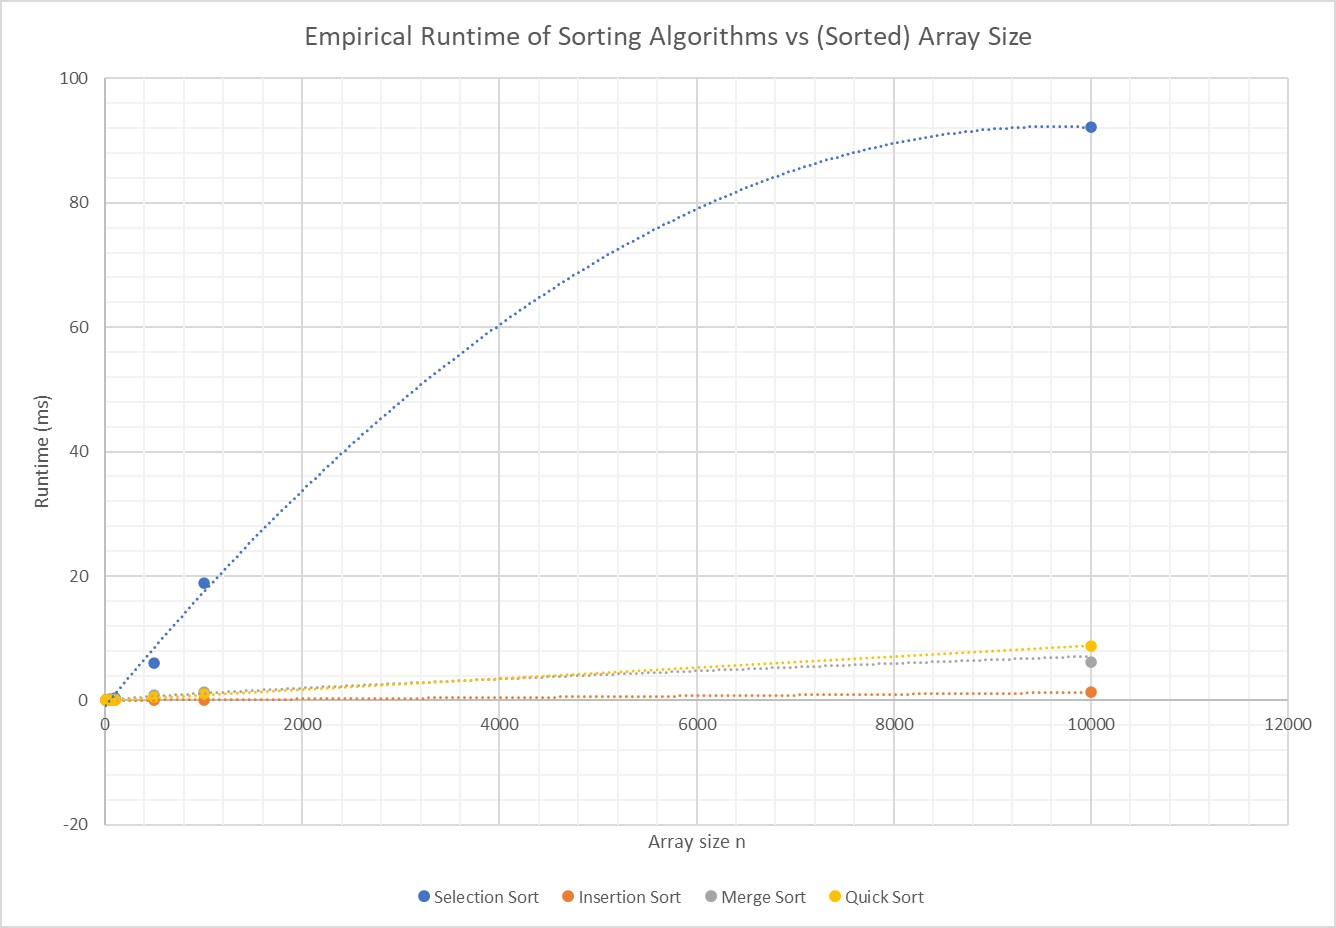
\includegraphics[scale=0.8]{sorted.jpg}
\hspace*{\fill}
\caption{Runtime vs Array Size for Different Sorting Algorithms on Sorted Arrays}
\label{fig:sorted}
\end{figure}
\end{center}

\begin{table}[H]
$$\begin{array}{|c|c|c|c|c|c|c|c|}\hline
\textbf{Algorithm} & n=5 & n=10 & n=50 & n=100 & n=500 & n=1000 & n=10000 \\ \hline
\text{Selection Sort} & 0.0033 & 0.0047 & 0.1489 & 0.6176 & 7.0836 & 15.7926 & 426.9315 \\ \hline
\text{Insertion Sort} & 0.0041 & 0.027 & 0.1019 & 0.8575 & 6.061 & 21.7456 & 480.8993 \\ \hline
\text{Merge Sort} & 0.0117 & 0.0248 & 0.1137 & 0.2024 & 0.9694 & 1.9961 & 8.3756 \\ \hline
\text{Quick Sort} & 0.0087 & 0.026 & 0.0568 & 0.101 & 0.5829 & 1.2182 & 6.4635 \\ \hline
\end{array}$$
\caption{Runtime Performance of Random Sorted Numbers in Descending Order}
\label{table:descending}
\end{table}
\end{center}

\begin{center}
\begin{figure}[H]
\hfill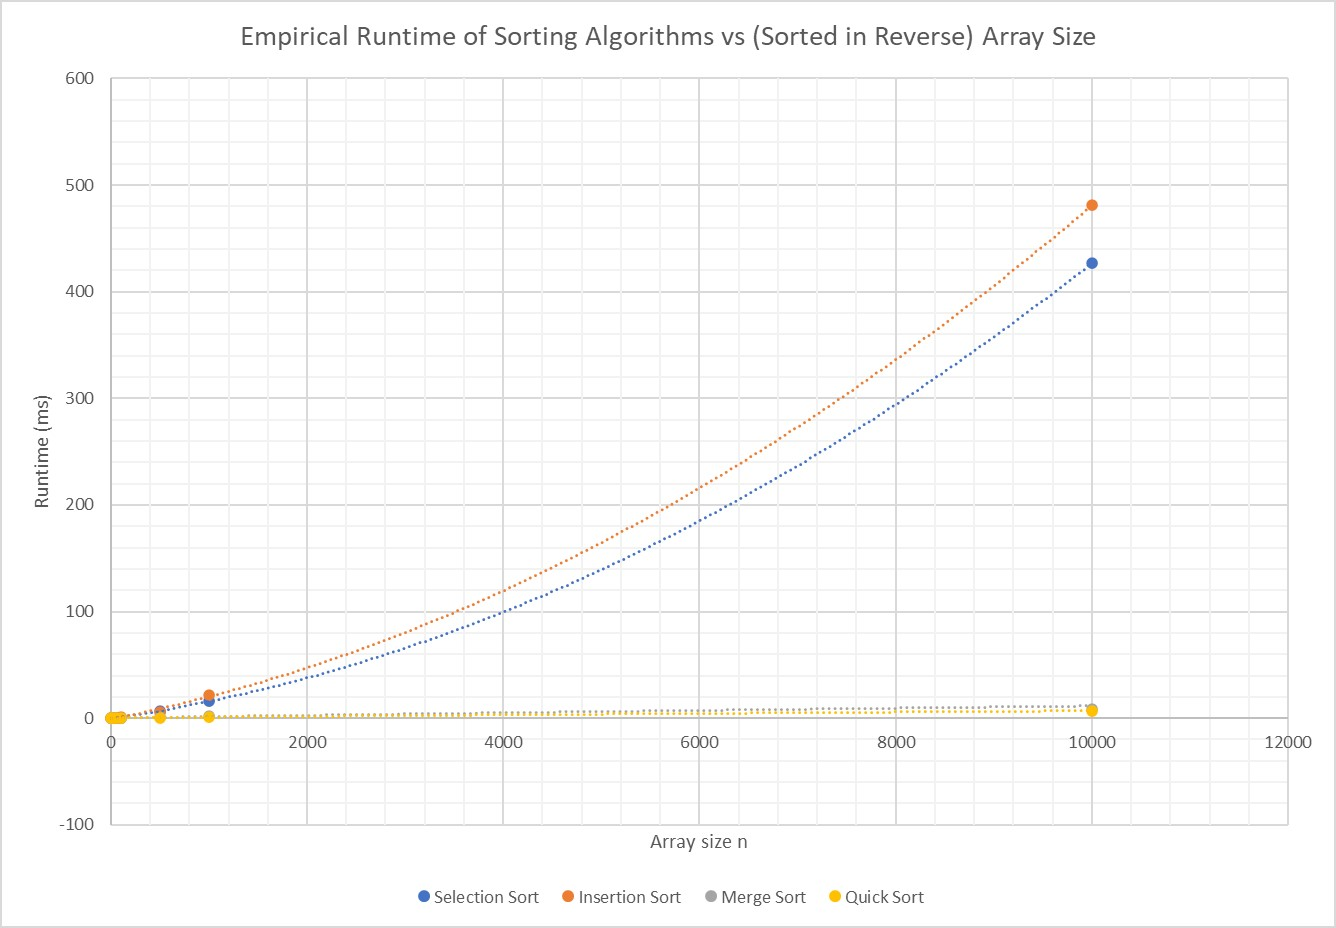
\includegraphics[scale=0.8]{reverse.jpg}
\hspace*{\fill}
\caption{Runtime vs Array Size for Different Sorting Algorithms on Sorted Arrays (In Reverse Order)}
\label{fig:reverse}
\end{figure}
\end{center}

Let $n$ denote the size of any given array.

For unsorted arrays, we observed that when $n$ was small, selection sort and insertion sort were faster than merge sort and quick sort. This is expected due to the recursion overhead produced by merge and quick sort. This overhead is less of an issue for larger arrays, as selection and insertion sort are both $O(n^2)$, whereas merge sort, and quick sort (given the fact that the median element is clearly a ‘good’ pivot as the partition lengths must always be $\le\frac{3n}4$) are both $O(n\log{n})$, and thus as expected, merge and quick sort were much faster for larger arrays.

Interestingly, merge sort was faster than quick sort for larger arrays, but slower for smaller arrays. This is likely because merge sort usually makes more recursive calls and thus produces more overhead. Also, quick sort operates under tail recursion, thereby optimising this issue. For larger arrays, clearly both algorithms will have many recursive calls, but on each call, quick sort has more operations due to the number of while loops to iterate through.

Generally, we observed selection sort to be slower than insertion sort, although this trend was not as clear-cut for smaller arrays. This trend is likely because selection sort continually scans the entire array, whereas insertion sort only needs to inspect  the unsorted region, hence requiring fewer operations. This also explains why in sorted arrays, selection sort was significantly slower than the other algorithms, and why insertion sort was the fastest algorithm in this scenario.

Regarding reversed arrays, similar, but less consistent trends were observed compared to randomly unsorted arrays. This is expected as this is simply the worst-case scenario of all sorting algorithms, whereas the sorted case is typically the best-case scenario.

Figure \ref{fig:code} presents the code used to calculate runtimes of different test cases.

\begin{figure}[H]
\begin{lstlisting}
import java.util.Arrays;
import java.util.Collections;
import java.util.Random;
import java.util.function.BiConsumer;

public class PerformanceAnalysis {

    public static Integer[][] generateArrays(Random generator, boolean sorted, boolean reverse,
            int length) {
        // Make 4 copies of array to be sorted (one for each algorithm to sort)
        Integer[][] toSort = new Integer[4][length];

        for (int i = 0; i < length; i++) {
            toSort[0][i] = generator.nextInt();
        }
        for (int j = 0; j < 4; j++) {
            toSort[j] = Arrays.copyOf(toSort[0], length);
            if (sorted && reverse) {
                Arrays.sort(toSort[j], Collections.reverseOrder());
            } else if (sorted) {
                Arrays.sort(toSort[j]);
            }
        }
        return toSort;
    }

    public static long testSort(Integer[] toSort, BiConsumer<Integer[], Boolean> algorithm) {
        long start, end;

        // Convert to milliseconds in Excel to prevent round-off error
        start = System.nanoTime();
        algorithm.accept(toSort, false);
        end = System.nanoTime();

        return end - start;
    }

    public static void main(String[] args) {
        Random generator = new Random();

        // Change these parameters per test
        Integer[][] toSort = generateArrays(generator, false, false, 5);
        
        // To handle issues with inconsistent runtimes of whichever method is called first, call
        // all methods on a random array
        Integer[][] randomTest = generateArrays(generator, false, false, 7);

        SortingAlgorithms.selectionSort(randomTest[0], false);
        SortingAlgorithms.insertionSort(randomTest[1], false);
        SortingAlgorithms.mergeSort(randomTest[2], false);
        SortingAlgorithms.quickSort(randomTest[3], false);

        long elapsed;

        elapsed = testSort(toSort[0], SortingAlgorithms::selectionSort);
        System.out.println("Selection Sort: " + elapsed);

        elapsed = testSort(toSort[1], SortingAlgorithms::insertionSort);
        System.out.println("Insertion Sort: " + elapsed);

        elapsed = testSort(toSort[2], SortingAlgorithms::mergeSort);
        System.out.println("Merge Sort: " + elapsed);

        elapsed = testSort(toSort[3], SortingAlgorithms::quickSort);
        System.out.println("Quick Sort: " + elapsed);
    }
}

\end{lstlisting}
\caption{Runtime Analysis Code}
\label{fig:code}
\end{figure}
\end{document}